
\chapter{Experiments and results}
\label{sec:testFun}

\vspace{5pt}
\begin{remark}
\label{rem:plusminus}
The whole consideration leading to define CSFD was performed for
GOPs of finding local/global minimizers.
It can be easily reformulated for GOPs of finding
local/global maximizers for which the equivalent minimization problem
can be established.
In this case the landscape deterioration consists in "leveling hills" 
instead of "filling valleys".
The particular class of such maximization GOPs is associated with continuous
objectives (fitnesses) $F$ defined on compacts in $\mathbb{R}^N$.
In such cases we can set the new fitness as $- F$ plus the maximum value 
of $F$ over the search domain
in order to obtain the equivalent minimization problem.
\end{remark}


The aim of our experiments is to show the efficiency of the 
\textit{Cluster Supported Fitness Deterioration} CSFD in finding 
basins of attraction of local solutions.


\section{Genetic Engine}
\label{sec:genEng}
The CSFD strategy uses the \textit{Simple Evolutionary Algorithm} (SEA).
In contrast to the \textit{Simple Genetic Algorithm} (SGA), 
SEA uses a real values as a parameters of the chromosome
in populations without performing coding and encoding
process before calculates the fitness values of individuals 
(see e.g. \cite{Schaefer2007}).
Namely, SEA is more straightforward, faster and more efficient than SGA.


We use the standard genetic operators for real-valued representation:
\begin{itemize}
  \item Crossover: $Y=x_1 + N(mean, \sigma_c)(x_2 - x_1)$, where $x_1, x_2$ are
  individuals, $N(mean, \sigma_c)$ stands for the multivariate normal
  distribution, $mean = \frac{x_1 + x_2}{2}$ is a $[x_1, x_2]$ centroid, 
  $\sigma_c$ is the parameter used to control exploration 
  and exploitation of the SEA.
  \item Mutation: $y = x + N(0, \sigma_m)$, where $x$ is the individual to be
  mutated, $\sigma_m$ the configurable mutation parameter.
\end{itemize}

We want the genetic engine to be cheap and converge very quickly to local
solutions, so we may efficiently deteriorate found basins of attraction in 
subsequent iterations. It is advisable to use smaller populations, since the
goal during each run of the SEA is to locate only one peak. Also to improve the
convergence of the population maintained by SEA we use proportional selection and we increase the
exploitation capabilities of the SEA using proper parameters, usually:
$\sigma_c \in [0.1, 0.3]$, $\sigma_m \in [0.4, 1.0]$, depending on the problem.


\section{Test functions}
\label{sec:testFun}
In order to visualize the deterioration process we use 
three 2D test functions:
\begin{itemize}
  \item Simple trimodal:
  \begin{equation}
  \label{eqn:trimodal}
  \begin{array}{c}
  F(x)=2e^{-((x_1+1)^2+(x_2+1)^2)} + 1.5e^{-((x_1-1.1)^2+x_2^2)} +
  4e^{-3((x_1+1.5)^2+(x_2-1.5)^2)}
  \end{array}
  \end{equation}
  for $x_1, x_2 \in [-4, 4]$.
  \item Rastrigin: 
  \begin{equation}
  \label{eqn:Rastrigin}
  \begin{array}{c}
  F(x)= 20 + \sum_{i=1}^2 (\, x_i^2 - 10 cos(2 \pi x_i) \, )
  \end{array}
  \end{equation}
  for $x_1, x_2 \in [-4, 4]$.
  \item Langermann:
  \begin{equation}
  \label{eqn:Langermann}
  \begin{array}{c}
  F(x) = \sum_{j=1}^5 c_j \,
  exp(\, - \, \frac{1}{\pi}
  ( \, (x_1 - a_j)^2 + (x_2 - b_j)^2 \, ))\\ 
  \\
  cos(\, \pi \, ((x_1 - a_j)^2 + (x_2 - b_j)^2 \, )) + 5,\\ 
  \\ 
  a = (3,5,2,1,7), \, b = (5,2,1,4,9), \, c = (1,2,5,2,3)
  \end{array}
  \end{equation}
  for $x_1 \in [0, 4], \, x_2 \in [-1, 3]$.
  \item Griewangk:
  \begin{equation}
  \label{eqn:Gierwangk}
  \begin{array}{c}
  F(x)=\frac{1}{4000} \, \sum_{i=1}^2 \, x_i^2 \, - \, \Pi_{i=1}^2
  \, cos \left( \frac{x_i}{\sqrt{i}} \right) + 1
  \end{array}
  \end{equation}
  for $x_1, x_2 \in [-4, 4]$.
\end{itemize}

W decide to handle maximization GOPs associated with benchmarks
(\ref{eqn:trimodal}), (\ref{eqn:Rastrigin}), (\ref{eqn:Langermann}),
(\ref{eqn:Gierwangk}) because their results can be more
expressively presented than the equivalent minimization ones. 
The CSFD instance dedicated to maximization problems
were utilized (see Remark \ref{rem:plusminus}).


\section{CSFD initial parameters}
\label{sec:InitPar}


In each of the tests we use the same set of initial values for algorithm's
parameters. The \textit{Cluster Supported Fitness Deterioration} needs the
following parameters to be configured: 
\begin{itemize}
  
  \item $popSize$ -- population size of the genetic engine used in CSFD;
  it is advisable to use small population to minimize the fitness computation
  costs; usually: $40 \, \leq \, popSize \, \leq \, 100$
  
  \item $\epsilon$ and $minPts$ -- OPTICS generating distance and minimum number
  of points in $\epsilon$-neighborhood (see Section \ref{sec:OPTICS});
  the values for the $\epsilon$ should be 'large enough' to allow
  the creation of proper \textit{ordering}, usually $\epsilon \in [0.5, 1.0]$
  depending on the selection pressure. $minPts$ should be chosen as follows:
  \begin{equation}
  \label{eqn:minPts}
  minPts = \left\{
  \begin{array}{ccc}
  \frac{popSize}{4} & \text{if} & 10 \leq \frac{popSize}{4} \leq  20\\
  10 & \text{if} & \frac{popSize}{4} < 10\\
  20 & \text{if} & 20 < \frac{popSize}{4}
  \end{array}
  \right.
  \end{equation}
  
  \item $\sigma_c \; \text{and} \; \sigma_m$ -- standard
  deviations used for the \textit{crossover} and \textit{mutation} respectively
  (see Section \ref{sec:genEng})
  
  \item $mutationProb$ -- mutation probability (crossover is always performed)
   
\end{itemize}

\section{Efficiency measures and CSFD results}
\label{sec:Measures}
We will use two simple measures in order to evaluate the deterioration
quality. The first one was the number of recognized basins of
attraction $NBA$.
The basin of attraction of the local maximizer is considered as recognized
by CSFD if the cluster of individuals was established and 
the cluster extension is fully included in the basin.


The second measure, called the degree of deterioration $DoD$, is
defined by the following formula:
\begin{equation}
\label{eq:dod}
DoD = \frac{F_0^{max} - F_M^{max}}{F_0^{max} - F_0^{min}}
\end{equation}
where $M$ is the number of iterations performed by the CSFD strategy, 
$F_0^{max}$ denotes the maximum value of the fitness at the beginning of the 
algorithm ($0$-iteration), similarly $F_0^{min}$ is the minimum value of the
fitness function at the beginning of the algorithm and $F_M^{max}$ is the 
maximum value of the fitness in the last iteration of the algorithm.
$DoD$ might be also expressed in percentage.

CSFD was run several times for each of the objective (\ref{eqn:trimodal}),
(\ref{eqn:Rastrigin}), (\ref{eqn:Langermann}), (\ref{eqn:Gierwangk}).
The most typical behavior of this strategy in case of each objective
are depicted in Figures \ref{fig:3modTest},
\ref{fig:rastriginTest}, \ref{fig:langermannTest}, \ref{fig:griewangkTest}.
Moreover Table \ref{tab:resultsCsfd} gathers the metrics values for these
computations.

The best performance was obtained for the Trimodal and Griewangk
benchmark for which all local maxima were encountered and for which the maximum degree 
of fitness leveling was obtained: $98\%$ and $84\%$ respectively.
All local maxima were also recognized in the case of the Rastrigin function,
but the degree of deterioration was only $64\%$. The Langermann benchmark
became most difficult for CSFD, since the degree of deterioration was only
$59\%$ and two basins of attraction (out of eighteen) remained unknown. 

Judging by the results of benchamrks (\ref{eqn:trimodal}),
(\ref{eqn:Rastrigin}), (\ref{eqn:Langermann}), (\ref{eqn:Gierwangk})
we see that our variant of sequential niching strategy called CSFD
is very efficient especially for highly multimodal problems with 
narrow basins of attraction (like the Rastrigin's function). This can
be attributed to the fact that solutions are found very quickly by the GA with
small, fast-converges populations and narrow basins of attraction are well
approximated by the crunching functions. We found all 64 solutions of the
Rastrigin's function in less than 70 iterations. However, what is an
advantage to one GOP is often a drawback to others which is
yet another conclusion from the \textit{No Free Lunch Theorem}.
For problems with small number of local solutions with broad basins of
attraction (like Griewangk's function) the CSFD performs way to many 
iterations before the global stop condition is fulfilled (see section
\ref{sec:TermConditions}) (69 iterations in case of Griewangk's function).
This happens because fast-convergence and small populations give very dense 
clusters and very 'narrow Gaussian bells' which depress only a part of the basin
and as a result the algorithm deteriorates one basin of attraction many times.
It can be very costly in high-dimensional domains where linear combination of 
many crunching functions may be computionally intensive.
The obvious solution to this problem would be to merge cluster extensions
belonging to the same basin of attraction once every $k$ iteration of the 
CSFD. $k$ should be explicitly given in the configuration of the
algorithm. However this method should be used very carefully as it may
destroy unexplored regions of the problem's domain.



\begin{table}
\begin{center}
\caption{Results of experiments (CSFD algorithm)}
\begin{tabular}{| l | c | r |}
\hline
\label{tab:resultsCsfd}
\textit{Function} & \textit{NBA} & \textit{DoD} \\ \hline \hline
Trimodal & 3/3 & 0.98 \\ \hline
Rastrigin & 64/64 & 0.64 \\ \hline
Langermann & 16/18 & 0.59 \\ \hline
Griewangk & 4/4 & 0.84 \\ \hline
\end{tabular}
\end{center}
\end{table}

\begin{figure}
  \centering
  \fbox{
    \includegraphics[scale=0.25]{csfd3mod/fitnessLand_iter000.jpg}
  }
  \fbox{
    \includegraphics[scale=0.25]{csfd3mod/fitnessLand_iter001.jpg}
  }
  \fbox{
    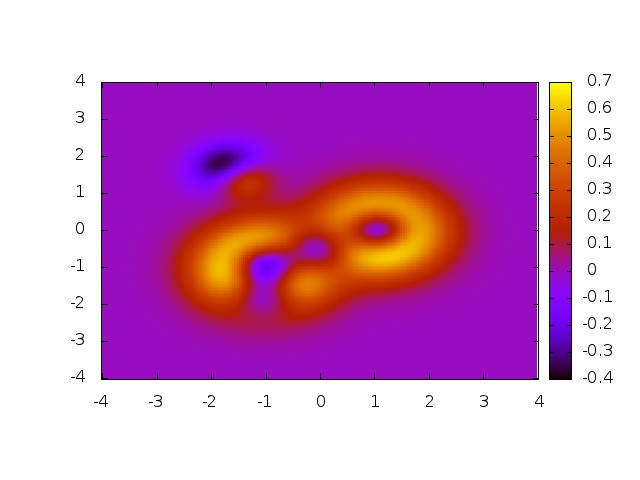
\includegraphics[scale=0.25]{csfd3mod/fitnessLand_iter005.jpg}
  }
  \fbox{
    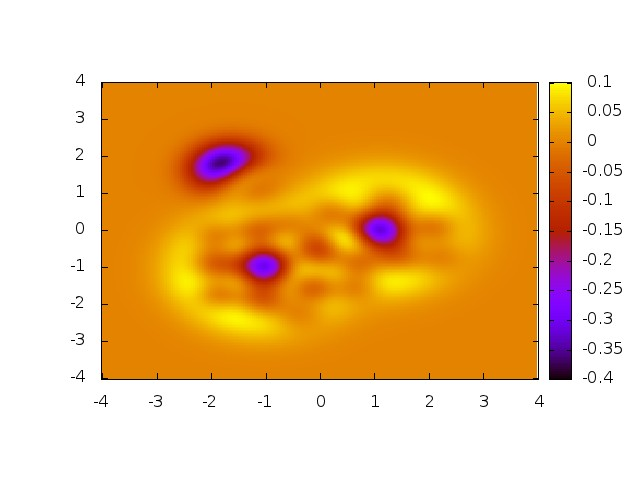
\includegraphics[scale=0.25]{csfd3mod/fitnessLand_iter020.jpg}
  }
  \caption{Original (left-up) and deteriorated fitness landscape 
  of the trimodal problem (function \ref{eqn:trimodal}) seen in the
  1th, 5th and 20th interation of the CSFD strategy respectively. 
  Parameters: $\epsilon=0.7$, $minPts=12$, $popSize=50$,
  $\sigma_c=0.1$, $\sigma_m=0.5$}
  \label{fig:3modTest}
\end{figure}

\begin{figure}
  \centering
  \fbox{
    \includegraphics[scale=0.25]{csfdRastrigin/fitnessLand_iter000.jpg}
  }
  \fbox{
    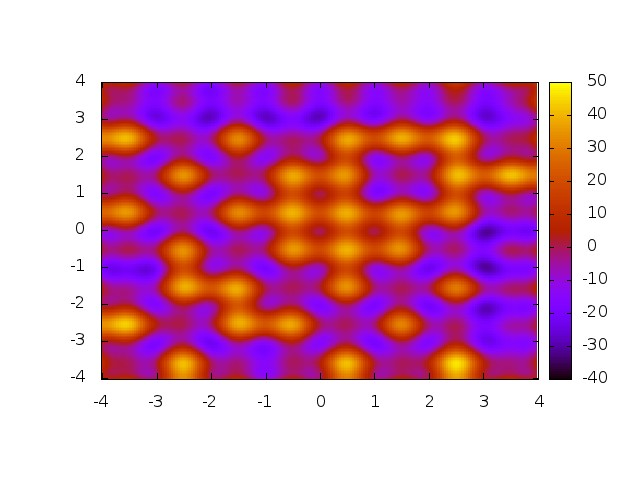
\includegraphics[scale=0.25]{csfdRastrigin/fitnessLand_iter033.jpg}
  }
  \fbox{
    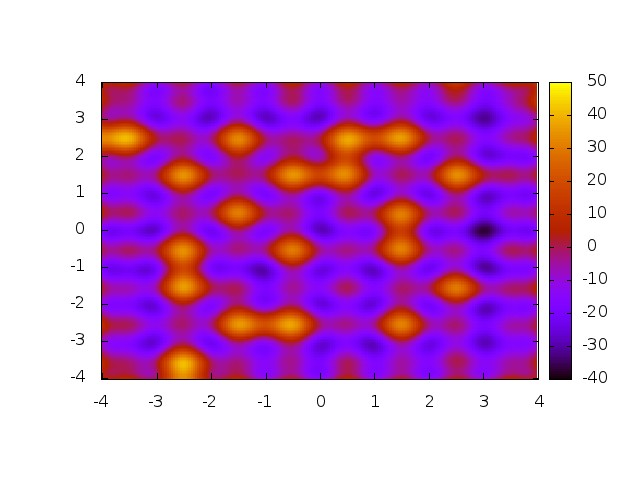
\includegraphics[scale=0.25]{csfdRastrigin/fitnessLand_iter045.jpg}
  }
  \fbox{
    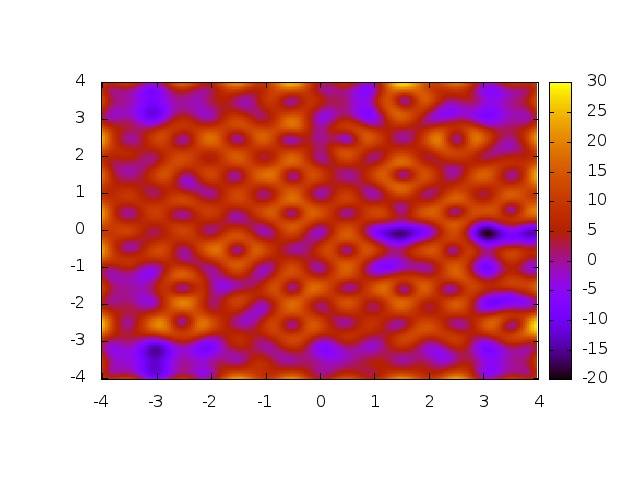
\includegraphics[scale=0.25]{csfdRastrigin/fitnessLand_iter064.jpg}
  }
  \caption{Original (left-up) and deteriorated fitness landscape 
  of the Rastrigin function (function \ref{eqn:Rastrigin}) seen in the 33th,
  45th and 64th interation of the CSFD strategy respectively. 
  Parameters: $\epsilon=0.7$, $minPts=12$, $popSize=50$,
  $\sigma_c=0.1$, $\sigma_m=0.5$}
  \label{fig:rastriginTest}
\end{figure}


\begin{figure}
  \centering
  \fbox{
    \includegraphics[scale=0.25]{csfdLangermann/fitnessLand_iter000.jpg}
  }
  \fbox{
    \includegraphics[scale=0.25]{csfdLangermann/fitnessLand_iter001.jpg}
  }
  \fbox{
    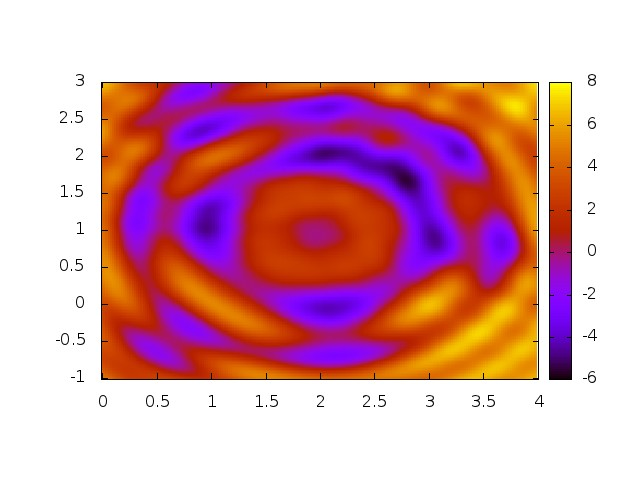
\includegraphics[scale=0.25]{csfdLangermann/fitnessLand_iter008.jpg}
  }
  \fbox{
    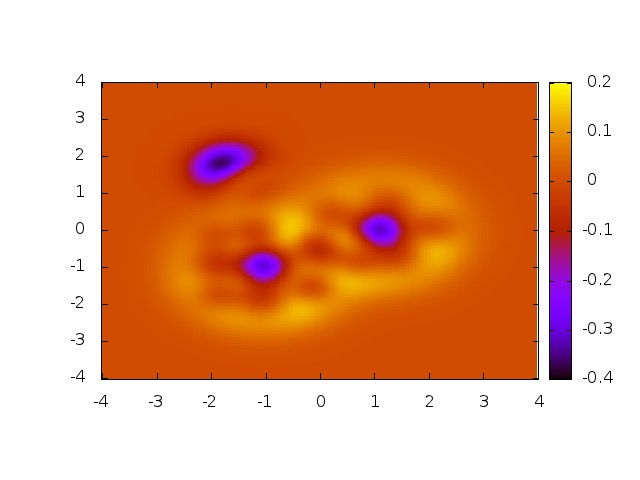
\includegraphics[scale=0.25]{csfdLangermann/fitnessLand_iter016.jpg}
  }
  \caption{Original (left-up) and deteriorated fitness landscape 
  of the Langermann function (function \ref{eqn:Langermann}) seen in the 1th,
  8th and 16th interation of the CSFD strategy respectively. 
  Parameters: $\epsilon=0.7$, $minPts=12$, $popSize=80$,
  $\sigma_c=0.1$, $\sigma_m=0.5$}
  \label{fig:langermannTest}
\end{figure}

\begin{figure}
  \centering
  \fbox{
    \includegraphics[scale=0.25]{csfdGriewangk/fitnessLand_iter000.jpg}
  }
  \fbox{
    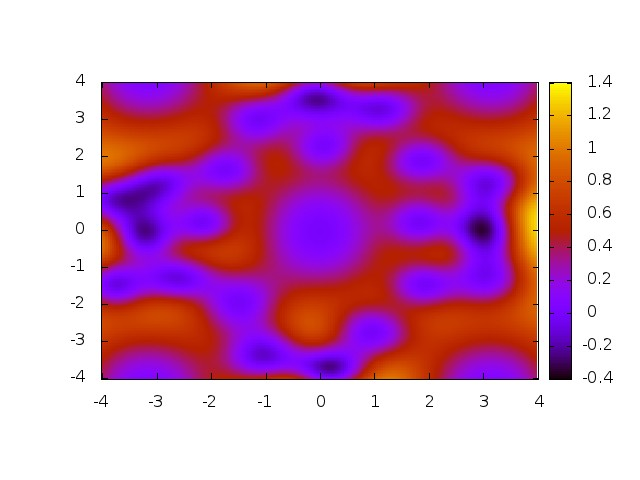
\includegraphics[scale=0.25]{csfdGriewangk/fitnessLand_iter021.jpg}
  }
  \fbox{
    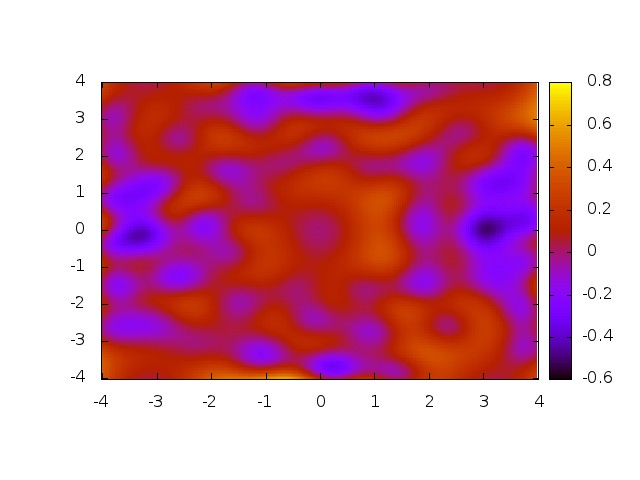
\includegraphics[scale=0.25]{csfdGriewangk/fitnessLand_iter051.jpg}
  }
  \fbox{
    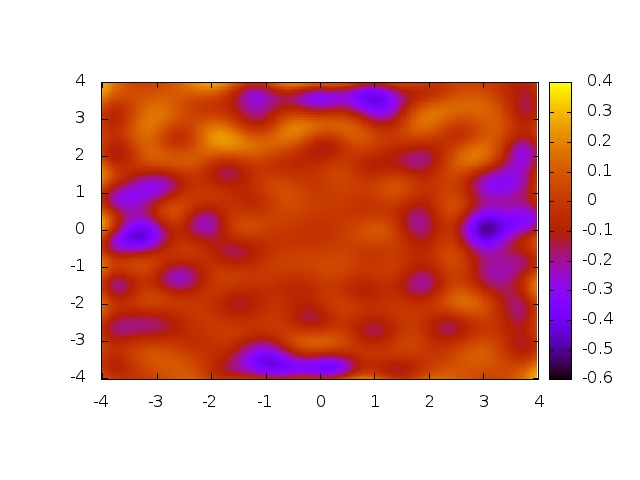
\includegraphics[scale=0.25]{csfdGriewangk/fitnessLand_iter069.jpg}
  }
  \caption{Original (left-up) and deteriorated fitness landscape 
  of the Griewangk function (function \ref{eqn:Gierwangk}) seen in the 21th,
  51th and 69th iteration of the CSFD strategy respectively. 
  Parameters: $\epsilon=0.7$, $minPts=12$, $popSize=50$,
  $\sigma_c=0.1$, $\sigma_m=0.5$}
  \label{fig:griewangkTest}
\end{figure}
